\documentclass[11pt,letterpaper,english]{article}
\usepackage[utf8]{inputenc}
\usepackage{tikz}
\usetikzlibrary{arrows}
\usetikzlibrary{calc}
\usepackage{amsfonts,amssymb,amsmath, amsthm}
\usepackage{color}
\usepackage{pgfplots}
\usepackage{pgfgantt}
\usepackage[colorlinks,urlcolor=black,citecolor=black,linkcolor=black,menucolor=black]{hyperref}

\begin{document}

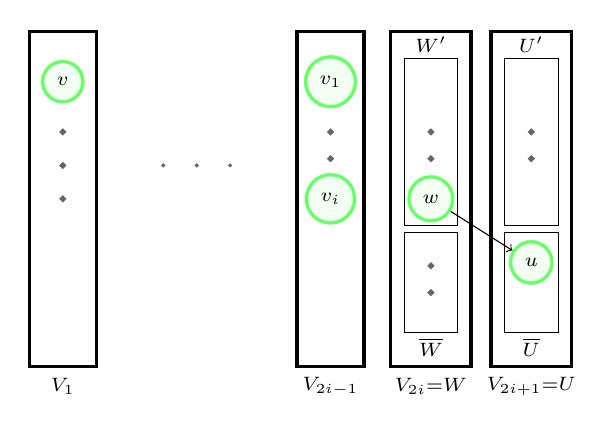
\begin{tikzpicture}
[scale=0.85,
 agent/.style={circle, draw=green!60, fill=green!5, very thick},
 good/.style={circle, draw=red!60, fill=red!5, very thick, minimum size=1pt},
]

\draw[black, very thick] (-0.5,-0.5-1) rectangle (0.5,3.5);

\node[agent]      (v) at (0,2.75)      {$\scriptstyle{v}$};

\filldraw[color=black!60, fill=black!5, very thick](0, 2) circle (0.02);
\filldraw[color=black!60, fill=black!5, very thick](0, 1.5) circle (0.02);
\filldraw[color=black!60, fill=black!5, very thick](0, 1) circle (0.02);

\node at (0, -0.5-1.30) {$\scriptstyle{V_1}$};

\draw[black, very thick] (-0.5+4,-0.5-1) rectangle (0.5+4,3.5);

\node[agent]      (v1) at (4,2.75)      {$\scriptstyle{v_1}$};
\node[agent]      (vi) at (4,2.75-1.75)      {$\scriptstyle{v_{i}}$};

\filldraw[color=black!60, fill=black!5, very thick](4, 2) circle (0.02);
\filldraw[color=black!60, fill=black!5, very thick](4, 1.6) circle (0.02);

\node at (4, -0.5-1.30) {$\scriptstyle{V_{2i-1}}$};

%W:
\draw[black, very thick] (-0.6+5.5,-0.5-1) rectangle (0.6+5.5,3.5);

%W'
\draw[black] (-0.5+5.6,0.6) rectangle (0.5+5.4,3.1);
\node at (5.5, 3.3) {$\scriptstyle{W'}$};
\node[agent]      (w) at (5.5,2.75-1.75)      {$\scriptstyle{w}$};

\filldraw[color=black!60, fill=black!5, very thick](5.5, 2) circle (0.02);
\filldraw[color=black!60, fill=black!5, very thick](5.5, 1.6) circle (0.02);


\draw[black] (-0.5+5.6,-1) rectangle (0.5+5.4,0.5);
\node at (5.5, -1.22) {$\scriptstyle{\overline{W}}$};

\filldraw[color=black!60, fill=black!5, very thick](5.5, 0) circle (0.02);
\filldraw[color=black!60, fill=black!5, very thick](5.5, -0.4) circle (0.02);


\node at (5.5, -0.5-1.30) {$\scriptstyle{V_{2i}=W}$};

%U:
\draw[black, very thick] (-0.6+7,-0.5-1) rectangle (0.6+7,3.5);

%U'
\draw[black] (1+5.6,0.6) rectangle (2+5.4,3.1);
\node at (5.5+1.5, 3.3) {$\scriptstyle{U'}$};

%U-bar
\draw[black] (1+5.6,-1) rectangle (2+5.4,0.5);
\node at (7, -1.22) {$\scriptstyle{\overline{U}}$};


\node[agent]      (u) at (7,2.75-2.7)      {$\scriptstyle{u}$};

\filldraw[color=black!60, fill=black!5, very thick](7, 2) circle (0.02);
\filldraw[color=black!60, fill=black!5, very thick](7, 1.6) circle (0.02);

\node at (7, -0.5-1.30) {$\scriptstyle{V_{2i+1}=U}$};

\draw[black,->] (w)--(u);


\filldraw[color=black!60, fill=black, thick](1.5, 1.5) circle (0.01);
\filldraw[color=black!60, fill=black, thick](2, 1.5) circle (0.01);
\filldraw[color=black!60, fill=black, thick](2.5, 1.5) circle (0.01);
\end{tikzpicture}

\end{document}